\chapter{Multi-output Habitat Mapping} \label{chap:dms}
On top of being able to produce probabilistic outputs, it would be of further advantage if preditions could be performed on multi-output data as well, to fully utilise the fact that many areas of the benthos will contain more than one label at any given time, where the simplifcation of these multi-labels to a single one thus far causes a considerable loss of information from the original data before the model fitting even begins. This is the motivation for us to explore Dirichlet multinomial distributions that have the ability to perform predictions over category counts, a perfect fit for the original data collected in this study.

Dirichlet multinomial regression, as the name suggestions, combines dirichlet and multinomial distributions to achieve the combined model. In particular, we are interested in modeling a distribution over category counts, as there exists relationship in our data such that every bathmetry point corresponds to a certain count of each possible label in the relevant area of benthos. To appreciate the Dirichlet Multinomial distribution as a whole, we briefly and describe the multinomial and Dirichlet distributions and the relationship, before delving into the equations needed to perform Dirichlet mulitnomial regression.

% \todo{explain why we should first revisit dirichlet, multinomial distributions separately before looking at dirichlet multinomial regression}

\section{Multinomial Distribution}
Multinomial distributions are the generalisation of binomial distributions that describe the probability of, for example, getting a heads or tails when flipping a two-sided coin. Generalising beyond $2$ categories, the multinomial does the same, but for any integer $n$ number of categories, like throwing an $n$-sided weighted die (weighted for the problem at hand). The relevance to the multi-label habitat data is then quite apparent, given that each data point needs to be mapped to any number of $K$ categories and sum to some number of samples stated. Draws from a multinomial distribution can be represented using a histogram such as that in \Cref{fig:exhist}. However, this particular histogram encapsulates the label distributions for the entirety of Scott Reef instead of what we actually want - a single coordinate.

\begin{figure}
    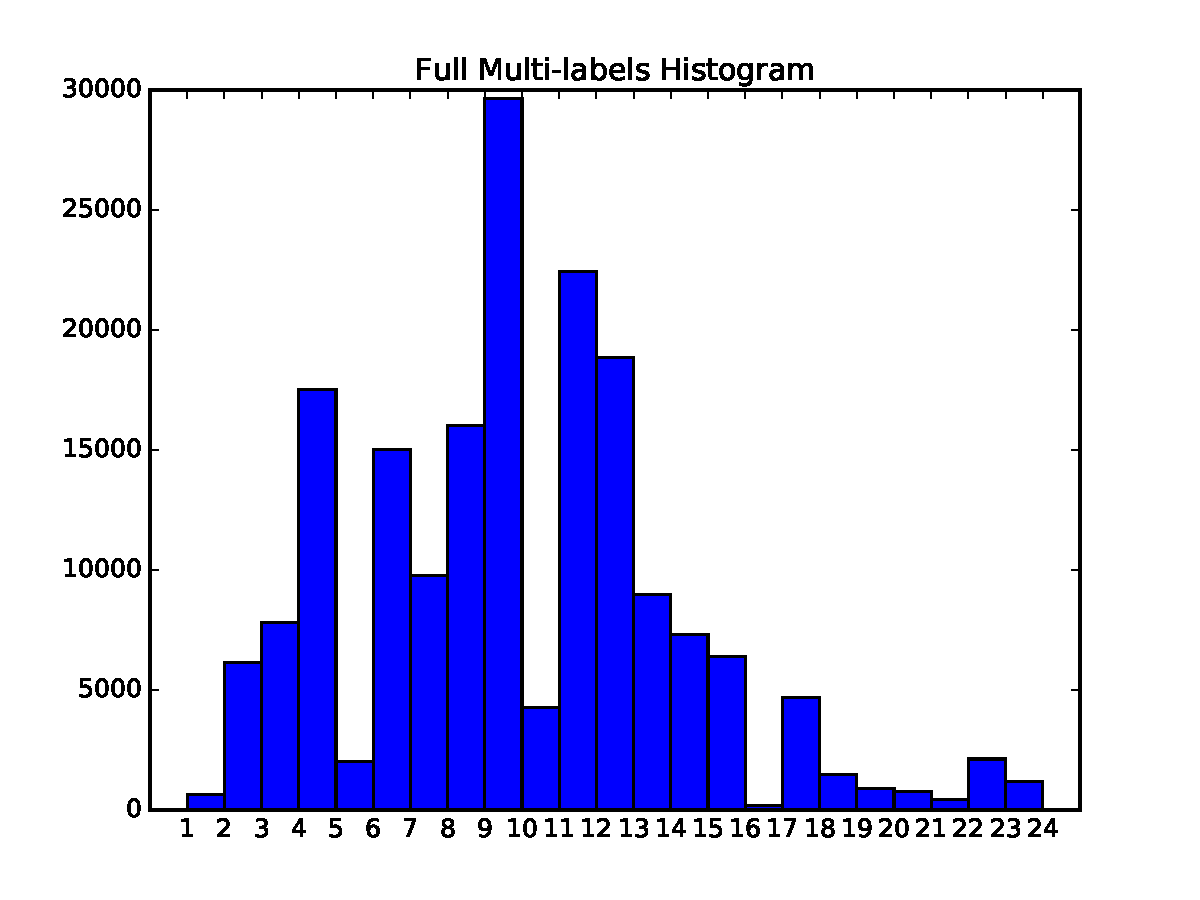
\includegraphics[width=\linewidth]{hist_full_multi_labels.pdf}
    \caption{Histogram of label counts for every multi-label data point}
    \label{fig:exhist}
\end{figure}

\section{Dirichlet Distribution}\label{chapsec:dirichlet}
To be able to perform predictions on individual points, it would seem that draws from a multinomial distribution need to be doable for a specific coordinate alone - but there does not exist the information to do so using the multinomial distribution alone, as a single vector of counts/draws as present in the multi-label data would be vastly insufficient. This is where the Dirichlet distribution comes in, placing a prior over the possible multinomial distributions. Parameters of the multinomial distribution can then be drawn from a Dirichlet given $\alpha$, the concentration parameters that govern the distribution of multinomial coefficients that can be drawn. The actual representation of a Dirichlet are $K$-dimensional vectors where $K$ is the number of possible categories where $\sum \mathbf{x} = 1$ for any vector $\mathbf{x}$, representing the distribution of $K$ labels that form the exhaustive set of possibilities, and hence sums to $1$. When working in $3$ dimensions, this can be represented visually on a triangle anchored at the unit coordinates along each of the $x, y, z$ axis (\Cref{fig:simplex}).

\begin{figure}
    \begin{minipage}{\linewidth}
        \centering
        \includegraphics[scale=0.7]{simplex.png}
        \caption*{Simplex plane in $3$-dimensional space}
    \end{minipage}
    \begin{minipage}{\linewidth}
        \includegraphics[width=\linewidth]{dirichlet_plots.png}
        \caption*{These three simplexes show the distributions of the multinomial coefficient draws for different values of $\alpha$, with the top showing the density of points using a heatmap, and the bottom plotting those points directly. When $\alpha=1$, the Dirichlet is equivalent to the uniform distribution. As $\alpha$ increases, the density of points towards a particular direction increasesas can be seen especially when comparing the second and third simplexes.}
    \end{minipage}
    \caption{}
    \label{fig:simplex}
\end{figure}

Given that the aim is to draw parameters for multinomial distributions from our Dirichlet, the following model is considered, where vectors $\mathbf{p}$ are the multinomial coefficients:
\begin{equation}
    \mathbf{p} | \mathbf{\alpha} = (p_1, \ldots, p_k) \sim \Dir(K, \mathbf{\alpha})
\end{equation}

The last important aspect of the Dirichlet distribution that needs to be looked at before moving onto the next section where the Dirichlet multinomial regression explained more formally, is calculating its entropy. Given the benefits of probabilistic output described in \Cref{chap:gps}, it would only make sense for a Dirichlet distribution to be able to provide simiilar information for vectors containing distributions over categories. This is done via its entropy: 

\begin{equation}
    \log \B(\alpha) - (k - \alpha_0) \psi(\alpha_0) - \sum_{j=1}^k(\alpha_j - 1)\psi(\alpha_j)
\end{equation}
where
\begin{equation}
    \B(\alpha) \frac{\Pi_{i=1}^k \Gamma(\alpha_i)}{\Gamma (\sum_{i=1}^k \alpha_i)}, \text{ and } \alpha_0 = \sum_{i=1}^k \alpha_i
\end{equation}

This would produce an entropy value for every vector of normalised category counts produced by the Dirichlet multinomial that can then be displayed using a heatmap over the same coordinates with query data for Scott Reef, providing a visual representation of entropy to allow easy identification of low entropy areas (higher confidence in predictions), compared to high entropy areas (higher variance in predictions and hence lower confidence).

% $$\theta \sim Dir(\alpha) \text{ , Dirichlet distributed random variable}$$ 
% $$p(\theta)= \frac{1}{\beta(\alpha)} \Pi_{i=1}^n \theta_i^{\alpha_i - 1} I(\theta \in S) \text{ density function, I is indicator function}$$ 
% $$ \theta = (\theta_1, ..., \theta_n), \alpha = (\alpha_1,...,\alpha_n), \alpha_i > 0 \text{ theta - n-dimensional vectors, alpha - parameters for distribution}$$
% $$ S = \{x \in R^n : x_i \geq 0, \sum x_i = 1\} \text{ S is probability simplex, the set of pmfs on numbers 1 through n}$$ 
% $$\frac{1}{\beta(\alpha)} = \frac{\Gamma(\alpha_0)}{\Gamma(\alpha_i) ... \Gamma(\alpha_n)}, \alpha_0 = \sum_{i=1}^n \alpha_i \text{ generalised beta function}$$

\section{Dirichlet Multinomial Regression}
Equipped with some basic knowledge about the Dirichlet and multinomial distributions, the steps involved in Dirichlet multinomial regression can be explained in context. The previous two sections looked at the two distributions in isolation - the aim now is to combine them in the Dirichlet multinomial, then optimise the parameters to be able to predict normalised category counts given training data, as previously described. The following formula is the joint prior distribution:

\begin{equation}
    \dirmul(C|\alpha) = \frac{M!}{\Pi_k C_k!} \frac{\Gamma(\sum_k \alpha_k)}{\Gamma(\sum_k c_k + \alpha_k)} \Pi_{k=1}^k \frac{\Gamma(C_k + \alpha_k)}{\Gamma(\alpha_k)}
\end{equation}
where $C$ are the category counts, $\alpha$ are the Dirichlet parameters as described in \Cref{chapsec:dirichlet}, and $M = \sum_k c_k$

The crucial part that has not yet been explained is how $\alpha$ is obtained/tuned to fit any training data available. In this study, the activation function chosen to calculate the $\alpha$ values was the softmax, also referred to as the `normalised exponential', in that it has better numerical stability than the exponential function \todo{(plot example if time allows)}. The softmax generalises the logistic function to $K$-dimensional data like that being used in this study:
\begin{equation}
    \alpha_k = \softmax{\mathbf{X}^T \mathbf{w_k}}
\end{equation}
where \begin{equation}
    \softmax(\mathbf{x})_i = \frac{e^{x_i}}{\sum_{j=1}^k e^{x_j}} \text{ for } i = 1, \ldots, K
\end{equation}

The weights $w$ here are in fact a matrix of weights with dimensions $(K \times D)$, where $K$ is the number of possible labels across the dataset, and $D$ is the dimensionality of the dataset. Muliplying the dirichlet multinomial prior by the Gaussian likelihood over weights then then gives the posterior that needs to be optimised to obtain the weights required to predict the normalised label counts at any given point:

\begin{equation}
    \Pi_{n=1}^N \dirmul (c_n | \alpha(x_n)) \times \Pi_{n=1}^k \sim \mathcal{N}(w_k | 0, \phi I)
\end{equation}
where $\phi$ is a regulariser that governs how much the weights $w$ are allowed to vary during the fitting process. To be able to optimise the weights, maximum a posteriori (MAP) estimation is used, which takes the set of parameters at the most likely point over the distribution. For example, in the $2$-dimensional example in \Cref{fig:MAP-ex}, the dotted line represents the value of $x$ that maximises the posterior distribution $P_{X|Y}(x|y)$.

\begin{figure}
    \includegraphics[scale=0.5]{MAP_example.pdf}
    \caption{Simple example of the MAP value for the posterior distribution over some variable $x$}
    \label{fig:MAP-ex}
\end{figure}

To perform MAP on the posterior distribution $P$, we take the log of $P$, as this scales the data in a way that allows optimisation algorithms working in multiple dimensions to determine how to search the space more efficiently:
\begin{multline}
    \log(P) = \sum^N_{n=1} [\log(M_k) - \sum_k \log(c_k!) + \log \Gamma(\sum_k \alpha_k(x_n)) - \log \Gamma(\sum_k c_{nk} + \alpha_k(x_n))] \\
    + \sum^N_{n=1} \sum^K_{k=1} [\log \Gamma(c_k + \alpha(x)) - \log \Gamma(\alpha_k(x_n))] \\
    + \sum^K_{k=1} [-\frac{\phi}{2} \log(2\pi \phi) - \frac{1}{2}w_k^T \phi \mathbb{I} w_k]
\end{multline}

To optimise this equation, the partial derivative of the above over the weights $w$ are considered:
\begin{multline}
    \partial \frac{\log p(c, x)}{\partial w_k} = \sum_{n=1}^N x_n \alpha_k (x_n) [\psi(\sum_l \alpha_l(x_n)) - \psi(\sum_k c_{nk} + \alpha_k(x_n))] \\
    + \sum^N_{n=1} x_n \alpha_k (x_n) [\psi (c_{nk} + \alpha_k(x_n)) - \psi(\alpha_k(x_n))] - \frac{1}{\phi} w_k
\end{multline}

% \todo {explain all the symbols here}

Given the log posterior and its partial derivatives over every weight, the MAP can then be calculated using parameter optimisation algorithms available in machine learning libraries \todo{(introduce this briefly the first time it comes up, in the GP section, then just to refer to that here.)}.

\subsection{Using Markov Chain Monte Carlo to Sample Weights}
Given the distribution of possible values of the weights $\mathbf{W}$ described, taking only the MAP for these values would be discarding other information in the distribution that also describes the data. While the MAP allows a single set of weights to be determined that allows performance to be assessed in addition to plotting maps to visualise the distribution of each habitat class in separate heatmaps, the `correctness' of the MAP estimation can further be assessed by generating maps created from weights from throughout the posterior distribution as they are drawn, then observing how consistent certain areas of the map remain when doing so.

To draw weights from the posterior distribution, Markov Chain Monte Carlo (MCMC) can be used. MCMC involves `random walks' through multiple dimensional space when using the Metropolis Hastings algorithm, where every step in $n$ dimensional space has a chance to be rejected or accepted. To account for the randomness in these walks (that provide \textit{chains} of parameters that the posterior is concerned with), Gelman-Rubin's r-hat statistic can be used to measure convergence when multiple MCMC instances are run for the same posterior. For multi-dimensional data, we will simply calculate the r-hat value for each dimension (each $w_{ij} in \mathbf{W} \text{ for } i=1,\ldots,K, j=1,\ldots,D$), and take their average.

\todo{(may need to explain MCMC and rhat in at least a little more detail here. at least include equation for r-hat statistic used})

% Using the MAP for optimisation, while a valid option, ignores all the possible weights in the given posterior distribution where they could also be drawn from. To create more certainty that the weights drawn from the distribution are in agreeance about the actual maps generated, MCMC would need to be used. By applying weights from the MCMC chains back to predictions and visually comparing differences, visual confirmation can be had on whether the maps remain reasonably consistent using weights drawn from the posterior.

\section{Illustrative Example}

The differences between a Gaussian Process that provides the probability distribution of possible labels compared to the Dirichlet Multinomial Regressor that provides the distribution of actual labels at a point, are highlighted in the illustrative example below. Three clusters A, B, C, over two labels were generated, such that B, C preferred labels $2, 1$, respectively, while cluster A contained an even mix of both - this can be observed by matching the colours of clusters to the adjacent colour bars.

% \todo{generate toy example with a mixed label A,B region and separate regions of mostly A, mostly B respectively}

\begin{figure}[H]
    \centerline{\includegraphics[scale=0.9]{toy_scattermap_clusters.pdf}}
    \caption{Plot of the synthesised data used. Only the {(x,y)} coordinates of the points are shown here, with actual label distributions shown below.}
    \label{fig:dm_toyplot}
\end{figure}

\begin{figure}[H]
    \centering
    \begin{minipage}{0.85\linewidth}
        \includegraphics[width=\linewidth]{toy_scattermap_0.pdf}
        \caption*{\textbf{Label distributions for label 1}, with mean distributions of $0.5, 0.1, 0.9$ for clusters A, B, and C respectively, observable from the colour bar.}
    \end{minipage}
    \begin{minipage}{0.09\linewidth}
        \includegraphics[width=\linewidth]{toy_scattermap_colourbar.pdf}
    \end{minipage}
    \begin{minipage}{0.85\linewidth}
        \includegraphics[scale=0.7]{toy_scattermap_1.pdf}
        \caption*{\textbf{Label distributions for label 2}, with mean distributions of $0.5, 0.9, 0.1$ for clusters A, B, and C respectively, observable from the colour bar.}
    \end{minipage}
    \begin{minipage}{0.09\linewidth}
        \includegraphics[width=\linewidth]{toy_scattermap_colourbar.pdf}
    \end{minipage}
\end{figure}

% \begin{figure}[H]
%     \includegraphics[trim={0 2cm 0 2cm}]{toyplot_hist_distr_legend.pdf}
%     \caption{Legend/axes for the following histogram plots showing distribution of labels at each point}
%     \label{fig:toyplothist_legend}
% \end{figure}

% \begin{figure}[H]
%     \begin{minipage}{.49\linewidth}
%         \includegraphics[width=\linewidth]{toy_clusterA_distr.pdf}
%         \caption{Label distribution of cluster A}
%         \label{fig:toyclusterA}
%     \end{minipage}
%     \hfill
%     \begin{minipage}{.49\linewidth}
%         \includegraphics[width=\linewidth]{toy_clusterB_distr.pdf}
%         \caption{Label distribution of cluster B}
%         \label{fig:toyclusterB}
%     \end{minipage}
%     \begin{minipage}{.49\linewidth}
%         \includegraphics[width=\linewidth]{toy_clusterC_distr.pdf}
%         \caption{Label distribution of cluster C}
%         \label{fig:toyclusterC}
%     \end{minipage}
% \end{figure}

In this example, the GP and DM models were each trained on half of each cluster, and made to predict the other half. However, as a standard GPC can only have single label inputs and outputs, a approximation/simplification was made for the purpose of calculating average error, whereby the label was simply taken to be the most frequently occurring label at any given point. While this is a reasonable simplification for clusters A, B as the dominant label has majority share, this is not the case for C, as the split between the two labels per point in the cluster is exactly even. 

\subsection{Results}

The results in \Cref{table:toy_gm_vs_gp} were taken from an average of $20$ runs. They show that the DM performed best when projecting the data to quadratic space, while the GPC did best on the original data as-is. This was taken into account for the plots below for the DM and GP respectively, which used an instance of the more favourably performing processed data. The DM plots below show the actual distributions for each label, allowing comparison with the true values, but the GP has taken the argmax of every label instead, as it cannot represent multi-label data.

\begin{table}[H]
    \label{table:toy_gm_vs_gp}
    \begin{tabular}{|C{4cm}|C{4cm}|C{6cm}|}
        \hline
        & Dirichlet Multinomial Regression RMSE* & Gaussian Process Classifier (argmax) RMSE \\\hline
        Original data & 0.0702 & 0.2683\\\hline
        Quadratic-space projection & 0.0656 & 0.4343\\\hline
        Cubic-space projection & 0.2902 & 0.4373 \\\hline
    \end{tabular}
    \begingroup
    \small{RMSE - root mean squared error}
    \endgroup
\end{table}

\begin{figure}
    \includegraphics[scale=0.85]{toy_scattermap_horz_colourbar.pdf}
    \begin{minipage}{\linewidth}
        \makebox[\textwidth]{
            \includegraphics[scale=.52]{toy_scattermap_test_expected_0.pdf}
            \includegraphics[scale=.52]{toy_scattermap_dmpreds_0.pdf}
        }
        \caption*{\textbf{Label 1} - expected (left) and predicted (right) label distributions.}
    \end{minipage}
    \begin{minipage}{\linewidth}
        \makebox[\textwidth]{
            \includegraphics[scale=.52]{toy_scattermap_test_expected_1.pdf}
            \includegraphics[scale=.52]{toy_scattermap_dmpreds_1.pdf}
        }
        \caption*{\textbf{Label 2} expected (left) and predicted (right) label distributions}
    \end{minipage}
    \caption{Coloured scatter maps of Dirichlet multinomial predictions. Where the yellow/green regeions appear to point to a discrepancy in predictions, it would be useful to refer to the colour bar to observe that yellow ($\approx0.9)$) is near to green, the lighter shades in particular ($0.75 \sim 0.85$)}
    \label{fig:toy_dmpredplots}
\end{figure}

\begin{figure}
    \begin{minipage}{\textwidth}
        \includegraphics[scale=0.75]{toy_scattermap_testgp_expected.pdf}
        \caption*{Expected labels from taking the most probable label per point}
    \end{minipage}
    \begin{minipage}{\textwidth}
        \includegraphics[scale=0.75]{toy_scattermap_gppreds.pdf}
        \caption*{Gaussian process predictions after taking the most probable label oer data point.}
    \end{minipage}
    \caption{Gaussian process expected and predicted scatter maps}
\end{figure}


% \begin{figure}[H]
%     \includegraphics[scale=0.6]{toy_dm_pred_plot0.pdf}
%     \caption{DM Label distribution of label 0}
%     \label{fig:toylabel0}
% \end{figure}
% \begin{figure}[H]
%     \includegraphics[scale=0.6]{toy_dm_pred_plot1.pdf}
%     \caption{DM Label distribution of label 1}
%     \label{fig:toylabel1}
% \end{figure} 
%\todo{dm - sitting on averages in each cluster. cause for concern?}

% \begin{figure}[H]
%     \includegraphics[scale=0.6]{gp_with_vars0.pdf}
%     \caption{OvR GP performance with variance for label 0}
%     \label{fig:toylabel0}
% \end{figure}
% \begin{figure}[H]
%     \includegraphics[scale=0.6]{gp_with_vars1.pdf}
%     \caption{OvR GP performance with variance for label 1}
%     \label{fig:toylabel1}
% \end{figure} 

\Cref{fig:toy_dmpredplots} shows that the DM was able to predict values close to the distributions in the original full clusters, with each the predictions in each clusters A, B with errors of $0.045$, while C increases slightly to $0.052$. The Gaussian process classifier was less consistent, however. Its accuracy in predicting the correct (argmax) label across all three clusters was $0.77$, where cluster A achieve an accuracy of $0.99$, cluster B $0.92$, but cluster C sharply dropped off to $0.416$ - given that this illustrative example only contains 2 classes, this corresponds to a predictive ability worse than random guess. 

\begin{figure}
    \makebox[\textwidth]{
        \includegraphics[scale=0.52]{toy_scattermap_dm_entropy.pdf}
        \includegraphics[scale=0.52]{toy_scattermap_gp_vars.pdf}
    }
    \caption{On the \textbf{left} are the plots of the \textbf{Dirichlet multinomial entropies} in clusters A, B, and C as indicated by the legend, and the same thing on the \textbf{right} for the \textbf{Gaussian process variances} (for simplicity, the the average of the two variances over each of the classes was taken). It is immediately noticable that while clusters A, B had low variance most of the time, cluster C's variance constantly remained unreasonably high. In comparison, the trend of the entropies in cluster C is higer than in A and B, but only by a small amount, and not remotely to the extent of the Gaussian proceses' variances.}
    \label{fig:dm-entr_vs_gp-vars}
\end{figure}

The Gaussian process' variance in the third cluster reinforces this fact - whereas the average variances in clusters A, B were only $0.076$ and $0.077$ respectively, it was $0.522$ in cluster C. On the other hand, the DM's confidence of a mixture of labels remains relatively stable (with a slight increase in entropy, however, with the average entropies in each cluster being $92, 87,$ and $101$ respectively.



% As we can see, the DM performed notably better than the GP, with the predictions in each cluster staying true to the original distributions. The GP, despite the $\sim 0.26$ error rate, can be seen to follow a consistent trend in the test data instead of adjusting to the two different classes. Most importantly, for both label 0, 1, the DM identifies that the portion of either label in cluster C is 0.5, due to its ability to learn and predict distributions at a point. As GPs are not designed to and cannot model this, it instead finds that neither label has a high probability, whilst also having a very high variance (beyond the $[0, 1]$ bound which again, the DM enforces but is not a property of a GP).

From this basic example, it is apparent that in the area where there is an even mix of labels A, B, the Gaussian Process' predictions are both noisy and very uncertain about their predictions, where human intervention would be required to observe the fact that it is in fact a consistent mix of both. In contrast, the dirichlet multinomial regressor is able to remain relatively confident of the fact that an area does in fact have a mix of labels.
